\chapter{Protostellar Disks and Outflows: Theory}
\label{ch:disks_theory}

\marginnote{
\textbf{Suggested background reading:}
\begin{itemize}
\item \href{http://adsabs.harvard.edu/abs/2014prpl.conf..173L}{Li, Z.-Y., et al. 2014, in ``Protostars and Planets VI", ed.~H.~Beuther et al., pp.~173-194}, sections 3-6 \nocite{li14a}
\end{itemize}
\textbf{Suggested literature:}
\begin{itemize}
\item \href{http://adsabs.harvard.edu/abs/2013MNRAS.432.3320S}{Seifried et al., 2013, \textit{MNRAS}, 432, 3320} \nocite{seifried13a}
\end{itemize}
}

The previous chapter introduced observations of protostellar disks and their outflows. This companion chapter reviews theoretical models of such disks, with particular attention to how they form, why they accrete, and why they launch outflows.

\section{Disk Formation}

\subsection{The Angular Momentum of Protostellar Cores}

To understand why disks form, we must start with the question of angular momentum. Stars form from protostellar cores, so we begin our study with the question of how much angular momentum cores typically contain. To determine this observationally, one maps a core in an optically thin tracer and measures the mean velocity on every line of sight through the core. If there is a systematic gradient in the mean velocity, that is indicative of some net rotation. Doing this for a sample of cores yields a distribution of rotation rates.

It is most convenient to express the resulting distribution dimensionlessly, in terms of the ratio of kinetic energy in rotation to gravitational binding energy. If the angular velocity of the rotation is $\Omega$ and the moment of inertia of the core is $I$, this is
\begin{equation}
\beta = \frac{(1/2)I\Omega^2}{a G M^2/R},
\end{equation}
where $a$ is our usual numerical factor that depends on the mass distribution. For a sphere of uniform density $\rho$, we get
\begin{equation}
\beta = \frac{1}{4\pi G \rho}\Omega^2 = \frac{\Omega^2 R^3}{3 G M}
\end{equation}
Thus we can estimate $\beta$ simply given the density of a core and its measured velocity gradient. Observed values of $\beta$ typically a few percent \citep[e.g.,][]{goodman93a}.

This implies that cores are not primarily supported by rotation. In fact, we can understand the observed rotation rates as being a property of the turbulence. Although cores are primarily thermally-supported, they do still have some turbulent motions present at transsonic or subsonic levels. Since most of the power in this turbulence is on large scales, there is likely to be a net gradient. When one performs the experiment of generating random turbulent velocity fields with a variety of power spectra and analyzing them as an observer would, the result is a $\beta$ distribution that agrees very well with the observed one \citep{burkert00a}.

\subsection{Rotating Collapse: the Hydrodynamic Case}

Given this small amount of rotation, how can we expect it to affect the collapse? Let us take the simplest case of a cloud in solid body rotation at a rate $\Omega$. Consider a fluid element that is initially at some distance $r_0$ from the axis of rotation. We will consider it to be in the equatorial plane, since fluid elements at equal radius above the plane have less angular momentum, and thus will fall into smaller radii.

Its initial angular momentum in the direction along the rotation axis is $j=r_0^2\Omega$. If pressure forces are insignificant for this fluid element, it will travel ballistically, and its specific angular momentum and energy will remain constant as it travels. At its closest approach to the central star plus disk, its radius is $r_{\rm min}$ and by conservation of energy its velocity is $v_{\rm max} = \sqrt{2 G M_*/r_{\rm min}}$, where $M_*$ is the mass of the star plus the disk material interior to this fluid element's position.
Conservation of angular momentum them implies that $j=r_{\rm min} v_{\rm max}$.

Combining these two equations for the two unknowns $r_{\rm min}$ and $v_{\rm max}$, we have
\begin{equation}
r_{\rm min} = \frac{r_0^4 \Omega^2}{G M_*} = \frac{4\pi \rho \beta r_0^4}{M_*},
\end{equation}
where we have substituted in for $\Omega^2$ in terms of $\beta$. This tells us the radius at which infalling material must go into a disk because conservation of angular momentum and energy will not let it get any closer.

We can equate the stellar mass $M_*$ with the mass that started off interior to this fluid element's position -- this amounts to assuming that the collapse is perfectly inside-out, and that the mass that collapses before this fluid element's all makes it onto the star. If we make this approximation, then $M_*=(4/3)\pi \rho r_0^3$, and we get
\begin{equation}
r_{\rm min} = 3 \beta r_0,
\end{equation}
i.e.\ the radius at which the fluid element settles into a disk is simply proportional to $\beta$ times a numerical factor of order unity.

We shouldn't take the factor too seriously, since of course real clouds aren't uniform spheres in solid body rotation, but the result that rotation starts to influence collapse and force disk formation at a radius that is a few percent of the core radius is interesting. It implies that for cores that are $\sim 0.1$ pc in size and have $\beta$ values typical of what is observed, they should start to become rotationally flattened at radii of several hundred AU. This should be the typical size scale of protostellar disks in the hydrodynamic regime.

\subsection{Rotating Collapse: the Magnetohydrodynamic Case}

Magnetic fields can greatly complicate this picture, due to magnetic braking. As a core contracts, rotation wants to spin it up, but this in turn twists up the magnetic field. This creates a tension force that opposes the rotation rate, and tries to keep the core rotating as a solid body.

To analyze this effect, let us work in cylindrical coordinates $(\varpi, \phi, z)$. Consider a fluid element in a disk at a distance $\varpi$ from the star, whose dimensions are $d\varpi$, $d\phi$, $dz$ in the $\varpi$, $\phi$, and $z$ directions. The fluid element is rotating around the star with a velocity $v_{\phi}$ in the $\phi$ direction. The fluid element is threaded by a magnetic field $\vecB=(B_\varpi, B_\phi, B_z)$. For future convenience we define the poloidal component of the field to be
\begin{equation}
\vecB_p = (B_\varpi, B_z),
\end{equation}
i.e., it is the component of the field not associated with wrapping around the rotation axis.

The $\phi$ component of the field is called the toroidal component, since it represents the part of the field that is wrapped in the rotation direction. If you drew a two-dimensional plot of the system in the $(\varpi, z)$-plane, the poloidal component would the one on the page, and the toroidal component would be the one into the page.

We will assume that both the fluid and the magnetic field are axisymmetric, so that they do not vary with $\phi$, although the field does have a $\phi$ component. The magnetic field exerts a Lorentz force per unit volume on the fluid element, given by
\begin{eqnarray}
\mathbf{f} & = & \frac{1}{4\pi} \left[(\nabla\times\vecB)\times \vecB\right] \\
& = & \frac{1}{4\pi} \left[\frac{B_\varpi}{\varpi} \frac{\partial(\varpi B_\phi)}{\partial \varpi} + B_z  \frac{\partial B_\phi}{\partial z}\right] \hat{\phi}\\
& = & \frac{1}{4\pi\varpi} \vecB_p \cdot \nabla_p (\varpi B_{\phi}) \hat{\phi},
\end{eqnarray}
where all the components except the $\phi$ one vanish by symmetry, and in the final step we have defined the poloidal gradient as $\nabla_p = (\partial/\partial\varpi, \partial/\partial z)$, i.e., it is just the components of the gradient in the $\varpi$ and $z$ directions.

The momentum equation, ignoring all components but those associated with the Lorentz force, is
\begin{equation}
\frac{\partial}{\partial t}(\rho \vecv) = \mathbf{f},
\end{equation}
so writing down the $\phi$ component of this equation and multiplying on both sides by $\varpi$, we have
\begin{equation}
\frac{\partial}{\partial t} (\rho v_{\phi} \varpi) = \frac{1}{4\pi} \vecB_p\cdot\nabla_p(\varpi B_\phi)
\end{equation}
The left hand side of this equation just represents the time rate of change of the angular momentum per unit volume $\rho v_{\phi} \varpi$, while the left hand side represents the torque per unit volume exerted by the field.

Given this equation, how quickly can a magnetic field stop rotation? We can define a magnetic braking time by
\begin{equation}
t_{\rm br} = \frac{\rho v_{\phi} \varpi}{\frac{\partial}{\partial t} (\rho v_{\phi} \varpi)}
= \frac{4 \pi \rho v_{\phi} \varpi}{\vecB_p \cdot\nabla_p (\varpi B_\phi)}
\end{equation}
To evaluate this timescale, consider the case of a fluid elements that is part of a collapsing cloud, and is trying to rotate at a velocity $v_{\phi}$ equal to the Keplerian velocity, i.e.
\begin{equation}
v_{\phi} = \sqrt{\frac{GM}{\varpi}},
\end{equation}
where $M$ is the mass interior to the fluid element.

If we started with a uniform cloud of density $\rho$, the mass interior to our element is $M\approx (4\pi/3) \rho \varpi^3$, so $v_\phi \approx \sqrt{(4\pi/3) G \rho \varpi^2}$. Plugging this into the timescale, we get
\begin{equation}
t_{\rm br} \approx \frac{(4\pi \rho)^{3/2} G^{1/2} \varpi^2}{\vecB_p \cdot\nabla_p (\varpi B_\phi)}
\end{equation}

To see what this at the order of magnitude level, let us suppose that the poloidal and toroidal components of the field are comparable, and that the characteristic length scale on which the field varies is $\varpi$, i.e.\ the field is fairly smooth on all scales smaller than the size of the region that is currently collapsing. In this case $\vecB_p \cdot \nabla_p (\varpi B_\phi) \sim B^2$, so the time scale we wind up with is
\begin{eqnarray}
t_{\rm br} & \sim & \frac{G^{1/2}\rho^{3/2} \varpi^2}{B^2} \\
& \sim & \frac{(G\rho)^{1/2} \varpi^2}{v_A^2} \\
& \sim & \frac{t_{\rm cr}^2}{t_{\rm ff}},
\end{eqnarray}
where we are dropping constants of order unity, in the second step we wrote $B$ in terms of the Alfven speed $v_A = B/\sqrt{4\pi \rho}$, and in the final step we wrote $t_{\rm cr} = \varpi/v_A$, where $t_{\rm cr}$ is the Alfven crossing time of the cloud.

\begin{marginfigure}
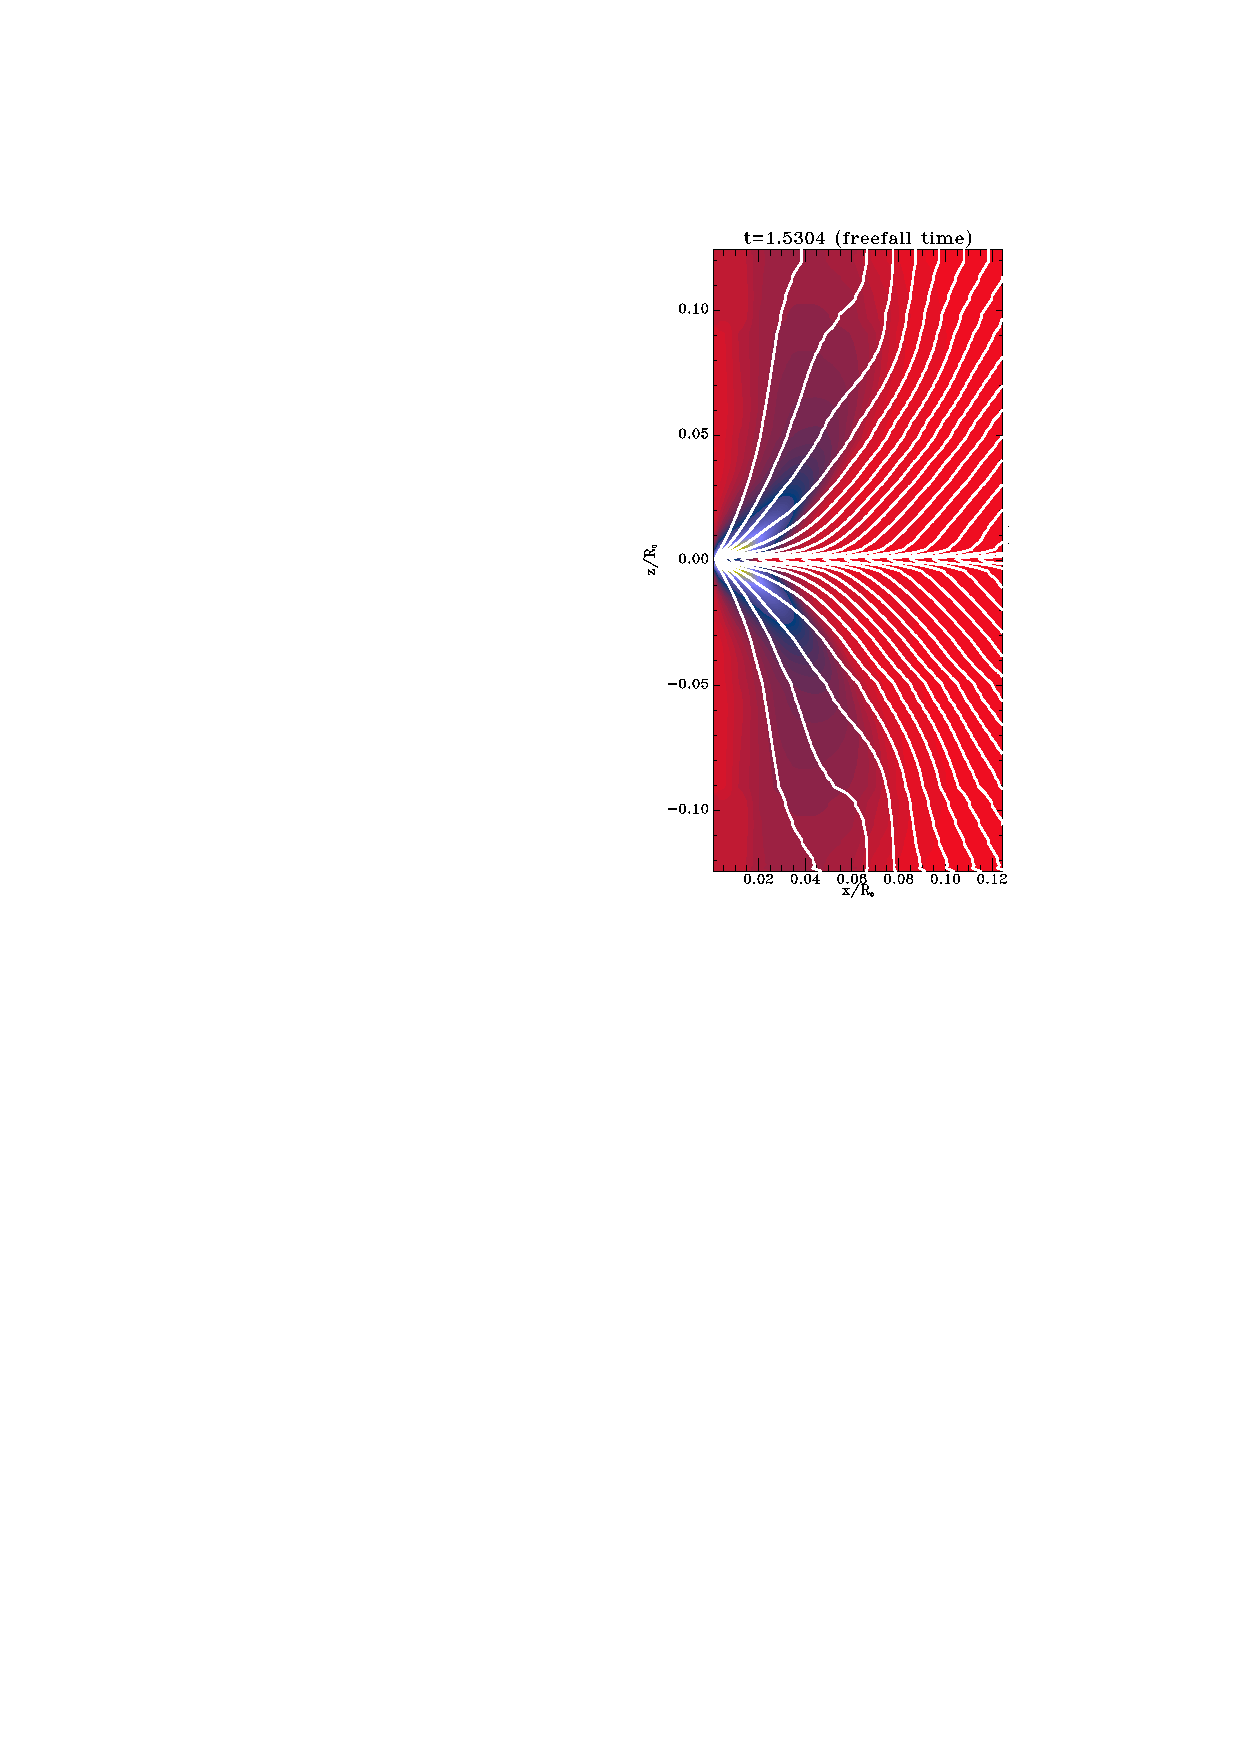
\includegraphics[width=\linewidth]{magdisk1_hennebelle08}
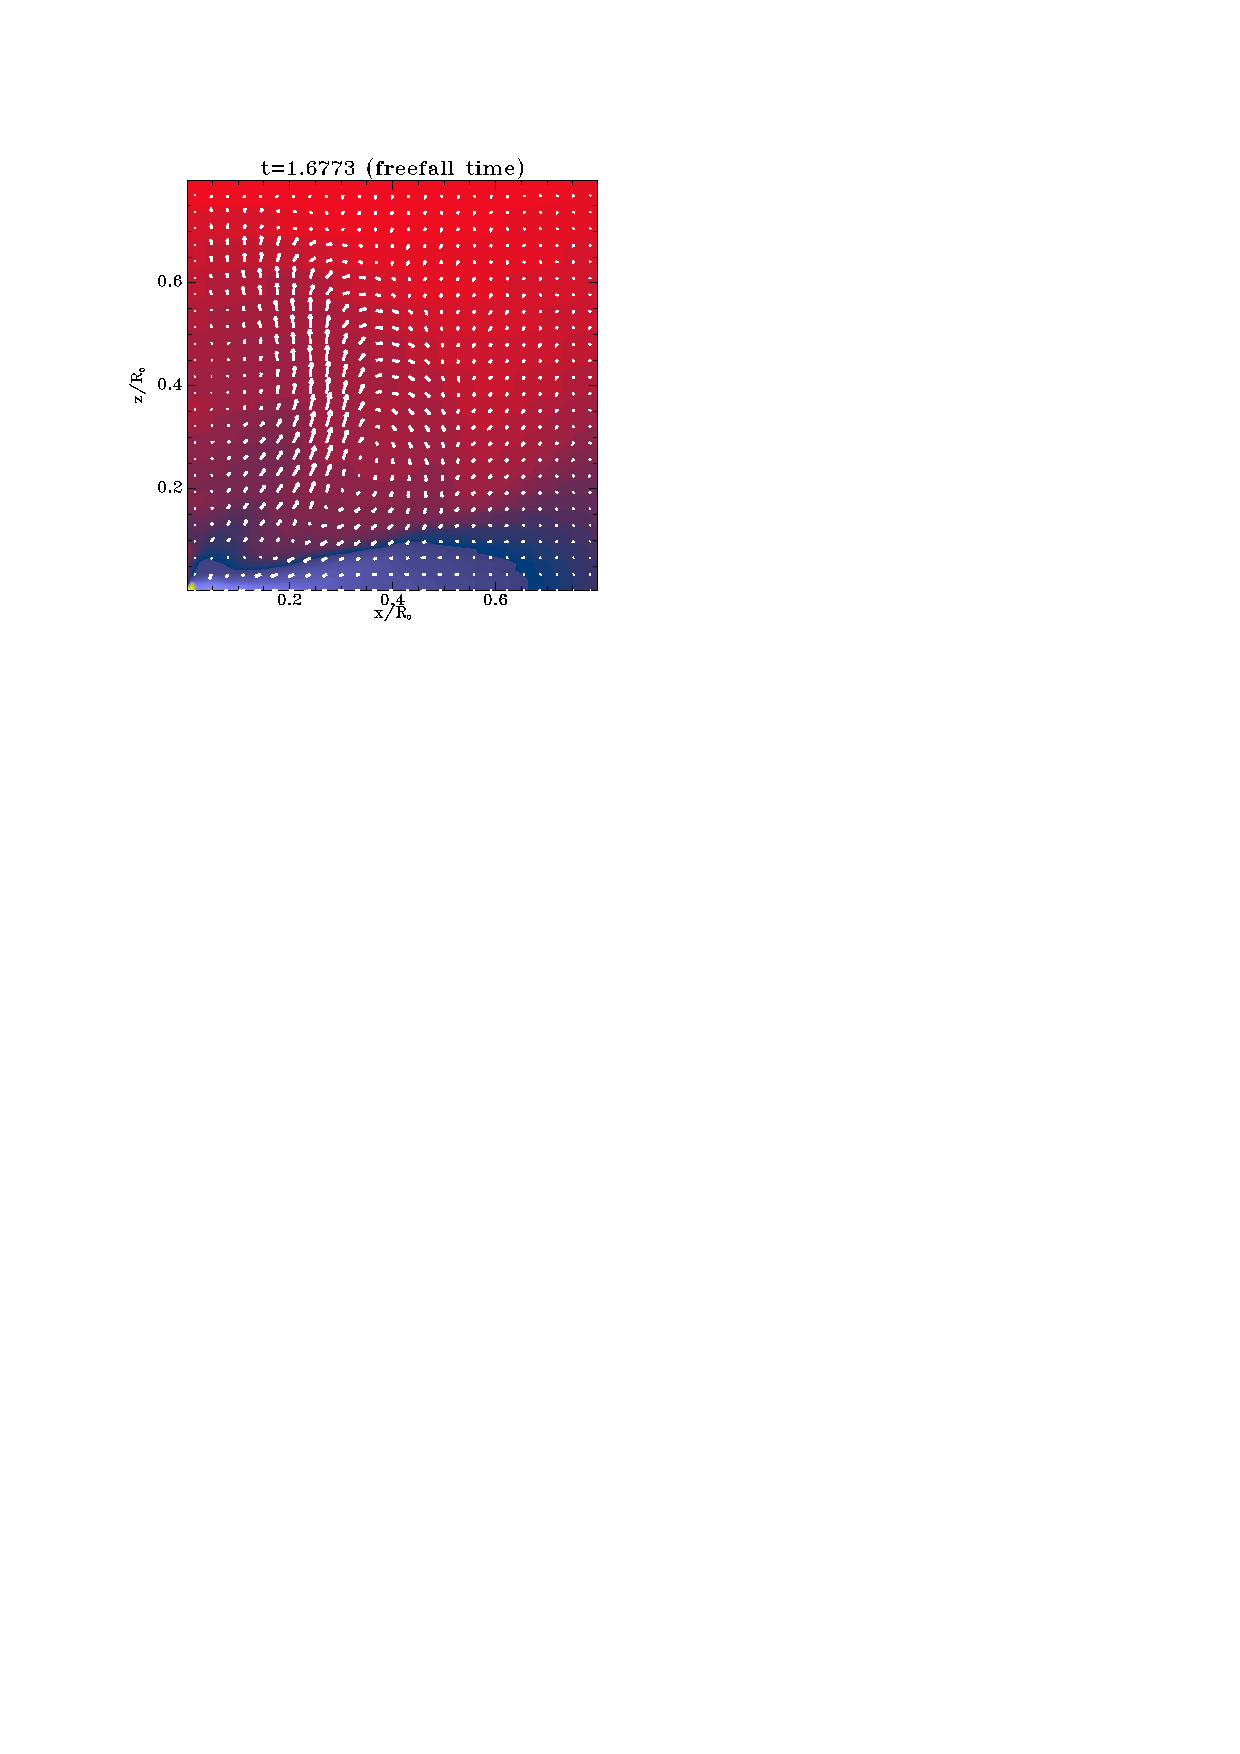
\includegraphics[width=\linewidth]{magdisk2_hennebelle08}
\caption[Simulations of magnetized rotating collapse]{
\label{fig:magdisk_hennebelle}
Results from a simulation of magnetized rotating collapse \citep{hennebelle08c}. The top panel shows the magnetic field structure; solid lines are poloidal magnetic field lines, while color indicates the azimuthally-averaged total magnetic field strength, on a scale from $0-3.5$ mG. The bottom panel shows the density (color) and velocity (arrows) structure at a slightly later time in the simulation. The structure in the mid-plane is a non-rotating pseudo-disk.
}
\end{marginfigure}

If a cloud starts out with a magnetic field near equipartition with gravity and thermal energies, we expect $t_{\rm ff} \sim t_{\rm cr}$, so this means that $t_{\rm br}\sim t_{\rm cr}$. This is an order of magnitude calculation, but its implication is clear: if we have a field that is even marginally wound up, such that the poloidal and toroidal components become comparable, this field is capable of stopping Keplerian rotation in a time scale comparable to the collapse or crossing time. This can effectively prevent formation of a Keplerian disk at all if the magnetic field is strong enough. Indeed, this is what simulations seem to show happening (Figure \ref{fig:magdisk_hennebelle}).

\subsection{The Magnetic Braking Problem and Possible Solutions}

The calculation of magnetic braking calculation we have just performed presents us with a fundamental problem: it naively seems like magnetic fields should prevent disks from forming at all, but we observe that they do. So how can we get out of this? This is not a completely solved problem, but we can make a few observations about what a solution might look like.

We can first ask whether ion-neutral drift might offer a way out. Recall in Chapter \ref{ch:magnetic}, we showed that, at the densities and velocities typical of protostellar cores, ion-neutral drift should allow gas to decouple from the magnetic field on scales below $L_{\mathrm{AD}} \sim 0.05$ pc. One might expect that this would make it possible to form disks below the decoupling scale.

